%\chapter{PARAMETERIZATION OF P CYGNI PROFILES DUE TO STELLAR WINDS} \label{chap:tool}
\chapter{TOOL FOR IDENTIFICATION OF SPECTRAL LINES IN XMM-NEWTON RGS SPECTRA} \label{chap:tool}
    %\doublespacing
    \minitoc
    \begin{center}
    	\emph{Abstract of chapter \ref{chap:tool}}
    \end{center}
    The identification of absorption and emission lines due to atomic species in the spectra of a X-ray binaries can reveal a wealth of information regarding the composition and physics of the stellar atmosphere. With the availability of high-resolution X-ray spectra from the RGS equipment on-board the XMM-Newton satellite, the study of such lines offers valuable diagnostics into the behaviour and evolution of the source object. Currently, data related to various atomic transitions, which lead to line formation, are made publicly available in the form of credible databases, one of them being the Atomic Spectra Database (ASD) at the National Institute of Standards and Technology (NIST). In this chapter, we present the development of a Python-based tool that accesses the relevant atomic data at NIST ASD for a given set of atomic species in a specific wavelength range and then overlays these lines on top of an X-ray spectrum obtained by the RGS spectrum of the XMM-Newton. With this tool, the astronomer can perform the important preliminary task of rudimentary line identification, before proceeding to advanced analysis of the X-ray data.
    
    \section{Introduction} \label{tool:intro}
    	XMM-Newton is an X-ray space observatory which was launched by the European Space Agency on December 10, 1999. It is designed to be a high throughput X-ray spectroscopy mission with spectral resolution of up to 0.025 \AA\ at 1 keV from the \textit{Reflection Grating Spectrometer} (RGS) detectors and an angular resolution of up to 1.1 arcsec from the \textit{European Photon Imaging Cameras} (EPIC) \cite{ehle2003xmm,jansen2001xmm}. With a bandpass of 5--38 \AA, corresponding to the energy range 0.33--2.5 keV, the spectra detected by RGS spans a substantial number of X-ray emission lines, which include the K-shell transitions and He-like triplets of light elements, such as C, N, O, Ne, Mg and Si, as well as the L-shell transitions of heavier elements like Fe and Ni. These factors enable the RGS spectra to be useful as diagnostic tools that can be used to investigate the physical conditions as well as the composition of the source of the spectra.
    
    \section{Working with RGS Data Files} \label{tool:rgs-files}
        The RGS spectra are available in the public domain in the \textit{Flexible Image Transport System} (FITS) file format \cite{chiappetti2018definition}, which is an open standard describing the digital file format for the storage, transmission and processing of data – formatted as multi-dimensional columns of tables. In spite of having the word `image' in its acronym, FITS files are most often used to store non-image data as well. This standard was designed, keeping in mind specifically astronomical data, namely images, spectra, lightcurves, photon lists, event lists, and source lists. In order to download the raw science data collected by XMM-Newton for any given source, there are two options:
        \begin{enumerate}[a)]
            \item By accessing the \textit{XMM-Newton Science Archive} (XSA) at the European Space Agency (ESA), using a web service (via a search form or a URL command access or methods from the \texttt{astroquery.esa.xmm\_newton} Python module) or by  \textit{table access protocol} (TAP) queries to the XSA database \cite{arviset2002xmm}.
            
            \item By accessing the \textit{High Energy Astrophysics Science Archive Research Center}, or HEASARC, at the National Aeronautics and Space Administration (NASA) using a web service \cite{barrett1993heasarc}.
        \end{enumerate}
        
        The XMM-Newton Science Operations Centre (SOC) provides a software package called the \textit{Science Analysis System} (SAS)\footnote{\url{https://www.cosmos.esa.int/web/xmm-newton/sas}}, which is a collection of tasks, scripts and libraries designed for the specific tasks of the reduction and analysis of the raw science data collected by the XMM-Newton observatory \cite{de2019users}. Using SAS, one can extract an RGS spectrum from the science data for a given X-ray source.
        
        An X-ray spectrum from RGS is found to contain a multitude of absorption and emission lines corresponding to atomic transitions in elements heavier than H and He. One of the initial and crucial tasks of the observer is to make a preliminary identification of the elemental lines at the wavelengths where they appear. This line identification also needs to incorporate the shift in the apparent position of the wavelength due to the Doppler effect. Currently, such line identification is performed by spectral-fitting programs such as Xspec or Spex while fitting the spectrum to prior theoretical models in which one can include the desired elemental abundances. However, when the spectrum used is of very high-resolution (such as that obtained from XMM-Newton), it often leads to poor fits, especially when one includes non-LTE model atmospheres. A Python-based tool was developed to address these deficiencies with the following motivation:
        \begin{enumerate}[a)]
            \item To upend the approach for fitting such high-resolution spectra by allowing the user to first quickly identify the prominent lines present in the spectrum as well the Doppler shift in the lines (if any).
            \item To estimate the elemental abundances (from the presence of specific lines) and the radial velocity of the emitting material (from the Doppler shifts).
            \item To allow the user to develop models for the individual lines and thereby engineer composite theoretical models which are more phenomenological as opposed to traditional approaches \cite{ness2020complications}.
        \end{enumerate}
        As present, while there are available codes that enable the parsing of atomic line data from NIST ASD (such as the \texttt{nist-asd} Python package on PyPI) or object-oriented interface for XSPEC (i.e. PyXspec), there is a lack of tools or codes that allow \textit{a priori} identification of spectral lines identification.
        
        In order get started, one first needs to obtain data of the atomic lines from credible databases, such as the \textit{Atomic Spectra Database} (ASD)\footnote{\url{https://www.nist.gov/pml/atomic-spectra-database}} at the \textit{National Institute of Standards and Technology} (NIST)\footnote{\url{https://www.nist.gov/}} \cite{ralchenko2008nist} and \textit{The Opacity Project online atomic database} (TOPbase)\footnote{\url{https://cds.unistra.fr/topbase/topbase.html}} \cite{cunto1993topbase}. To obtain this data, one may either use the web service provided to send queries to these databases, or one may use the relevant methods in various Python modules.
        
        Having identified the prominent lines in the RGS spectrum, one can then proceed to estimate the radial velocity of the source, the abundance of the elements in the emitting material and the interstellar absorption along the line-of-sight.
        
        \subsection{Extraction of RGS Spectra} \label{tool:rgs-files:extraction}
        
            \subsubsection{Obtaining source-specific science data} \label{tool:rgs-files:extraction:data}
                XMM-Newton data is publicly available at the online multi-mission science data archive known as HEASARC\footnote{\url{https://heasarc.gsfc.nasa.gov/}}. The easiest way to access relevant data for any specific source is by using its browse service\footnote{\url{https://heasarc.gsfc.nasa.gov/db-perl/W3Browse/w3browse.pl}} where one can enter the name of the source (or its right ascension and declination, if these are known) and the mission name (such as XMM-Newton or Chandra). One can supply additional information about the source as well, such as the observation dates. The more specific the query, the lesser would be the time taken to access and download the data.
                
                HEASARC provides the relevant data products in the form of a \texttt{.tar} file, which may then be extracted to obtain the \textit{Observation Data Files} (ODF), in case of XMM-Newton.
            
            \subsubsection{Reprocessing of science data} \label{tool:rgs-files:extraction:reprocess}
                The downloaded ODF files are compressed in \texttt{.gz} format and need to be extracted before reprocessing them using the software package SAS. Two SAS commands are used during the reprocessing – \texttt{cifbuild} and \texttt{odfingest}. While the former produces an index file of all the calibration data relevant to the specific source under consideration, the latter creates a summary file of the ODF using the house-keeping data files and the calibration database \cite{de2019users}.
                
                Subsequently, the data from both RGS instruments for the first and second spectral orders is extracted using the SAS task \texttt{rgsproc}. In five processing stages, this task extracts the events, the angles, the filter events, the spectra, the response matrices and the lightcurves.
        
        \subsection{Accessing Spectral Data from FITS Files} \label{tool:rgs-files:access}
            One of the outputs of the \texttt{rgsproc} task are two fluxed spectra -- one for each spectral order. Each of these files contain the spectra fluxed from both the RGS instruments. One must bear in mind that these fluxed spectra are inherently just a qualitative summary of the data, and should not be used for quantitative analysis. However, in the current work, because the objective is to merely aid the user in the identification of atomic lines -- which could be a preliminary step before serious spectral modeling, these fluxed spectra are more than sufficient as input files.
            
            \subsubsection{The \texttt{astropy} Python module} \label{tool:rgs-files:access:astropy}
                The fluxed spectrum file is saved in the FITS format. So the appropriate way to read its contents and extract the data is by using \texttt{astropy}\footnote{\url{https://www.astropy.org/}} \cite{robitaille2013astropy}, which is an open-source and community-developed Python package providing various functionalities that are important to astronomical applications.
                
                The \texttt{astropy.io.fits} package provides the user with access to FITS files. One first reads the list of \textit{header data units} (HDU), which is the highest level component of a FITS file -- consisting of a header and a table (or data array). This can be done using the \texttt{astropy.io.fits.open()} function which takes the FITS filename as input and returns an object of the \texttt{HDUList} class -- a list-like collection of HDUs.
            
            \subsubsection{Reading spectral data from FITS file} \label{tool:rgs-files:access:io}
                One can access the individual HDUs in a FITS file using the array indexing syntax -- the first index pointing to the primary HDU by default. For instance, if the object returned by the \texttt{astropy.io.fits.open()} function is named \texttt{hdul}, then \texttt{hdul[0]} would be the primary HDU, \texttt{hdul[1]} the first extension HDU and so on.
                
                In case of the fluxed spectra from RGS, the FITS files contain a single extension HDU corresponding to the spectrum -- accessed using \texttt{hdul[1]}, which is a table containing 3600 rows and 3 columns. Then the data attribute of \texttt{hdul[1]} (or \texttt{hdul[1].data}) would return a \texttt{NumPy} numerical array containing the channels/wavelengths (in \AA), the flux and the errors (both in s$^{-1}$cm$^{-2}$\AA$^{-1}$). The fluxes and errors corresponding to all bad channels contain \texttt{NaN} values, which can be filtered using the \texttt{isnan()} function and set to zero.
        
        \subsection{Collecting Atomic Lines} \label{tool:rgs-files:line-collection}
            In order to be able to identify atomic lines in a spectrum, one needs to have a line list that contains information about the lines present within a given wavelength range for all the ion stages of the atoms under consideration. With tremendous improvement in computing power, the various online databases of atomic data provide more accurate and updated information that may be used to built better line lists.
            
            So a code for qualitative atomic line identification in a spectrum becomes more reliable if it is able to access the current atomic data available online. This work achieves this objective by retrieving data for atomic transitions directly from ASD at NIST during runtime. So it is important to have an internet connection available while running the code for the first time or when one modifies the list of ions considered. As long as one keeps running the code subsequently on the same terminal session, using an unaltered ion list, the code would proceed to use the atomic data which is cached locally and one may work offline in that case.
            
            \subsubsection{The astroquery Python module} \label{tool:rgs-files:line-collection:astroquery}
                Atomic data from NIST can be accessed using the \texttt{astroquery} module\footnote{\url{https://astroquery.readthedocs.io/en/latest/}} \cite{ginsburg2019astroquery}, which uses the Python requests package for making HTTP requests and utilizes the data parsing functionality of the \texttt{astropy} package. The NIST ASD can be sent query requests and data retrieved therefrom using the \texttt{astroquery.nist} module.
            
            \subsubsection{Reading atomic line data from NIST} \label{tool:rgs-files:line-collection:NIST}
                The \texttt{astroquery.nist.Nist.query()} function provides an easy way to send HTML requests to NIST ASD. This function takes, as inputs, the lower and upper wavelength values and the name of the ion to be considered. One can also make use of the \texttt{astropy.units.AA} attribute to convert the wavelength value to \AA\ units.
                
                This function returns an object of the \texttt{astropy.table.Table} class. Then individual table rows can be accessed by the indexing syntax. The elements of a row can be subsequently accessed using the corresponding column header as a dictionary key. For instance, if the object named \texttt{ion\_table} stores the output of the \texttt{query()} function, then one can access the Ritz wavelength on the 17$^\text{th}$ row as \texttt{ion\_table[16]['Ritz']}.
        
        \subsection{Demonstration} \label{tool:rgs-files:demonstration}
            What follows is a demonstration of the developed tool using the flux spectrum of the galactic luminous supersoft X-ray source RX J0925.7-4758, which was discovered in the Galactic Plane Survey of the ROSAT All-Sky Survey \cite{motch1994}. The specific observations were made during 16--17 December 2000 with the RGS exposures being carried out for a duration of 61.2 ks \cite{motch02} under the observation ID 0111150101. The ODF files were downloaded from HEASARC and RGS data were processed using the SAS task \texttt{rgsproc} under default settings.
            
            For the identification of atomic lines for specfic ion stages present in the spectrum, the fluxed spectrum file named \texttt{P0111150101OBX000fluxed1000.FIT} (produced by \texttt{rgsproc}) is sufficient for the code to work. This specific file fluxes together the first-order spectra from both the RGS instruments. A copy of this file is provided with the distribution of the code for the user to reproduce the demonstrations that follow, as well as to try out variations of the run.
            
            Three specific Python scripts are provided with the distribution, whose outputs are presented in this work. A study of these scripts provides the user with an experience of how to use the methods developed in this work. All the scripts take, as the second command-line argument, the name of the file containing the fluxed spectrum. Briefly, these scripts perform the following tasks:
            
            \begin{enumerate}[i.]
                \item \texttt{line-overlaid-flux.py}: computes all the atomic lines within the wavelength range chosen and produces a plot of the fluxed spectrum with these lines overlaid.
                
                \item \texttt{flux-inspect.py}: allows the user to examine specific regions of interest, such as the vicinity of a known atomic line, within the chosen wavelength range.
                
                \item \texttt{line-shift.py}: displays the Doppler shifts in the Lyman $\alpha$, $\beta$, and $\gamma$ lines for the H-like and He-like C, N and O ions, as well as some common Fe ion lines.
            \end{enumerate}
        
            \subsubsection{Reading fluxed spectrum from FITS file} \label{tool:rgs-files:demonstration:read-flux}
                The use of the \texttt{astropy.io.fits} module is wrapped up in a method named \texttt{get\_flux}. This method takes a single argument, which is the name of the FITS file containing the fluxed spectrum -- in this case, the file named \texttt{P0111150101OBX000fluxed1000.FIT}. It returns the wavelengths (in \AA), the normalized flux and the error (both in s$^{-1}$cm$^{-2}$\AA$^{-1}$) in the form of three lists, which can be subsequently manipulated.
                
            \subsubsection{Preview of spectrum} \label{tool:rgs-files:demonstration:preview}
                When one is working with the spectrum of a new source, one may not be aware of the wavelength region which contains most of photon flux. Also, RGS spectra tend to have  a very low SNR in the small wavelengths up to $\sim$7 \AA. So, in order to help the user to ascertain a more pragmatic range, the function named \texttt{preview\_flux} quickly plots the entire spectrum. This method takes, as arguments, two lists -- the wavelengths in \AA~and the flux. The preview of the first-order fluxed RGS spectrum for RX J0925.7-4758 is shown in figure \ref{fig:spec-preview}.
                
                \begin{figure}[h!]
    				\centering
    				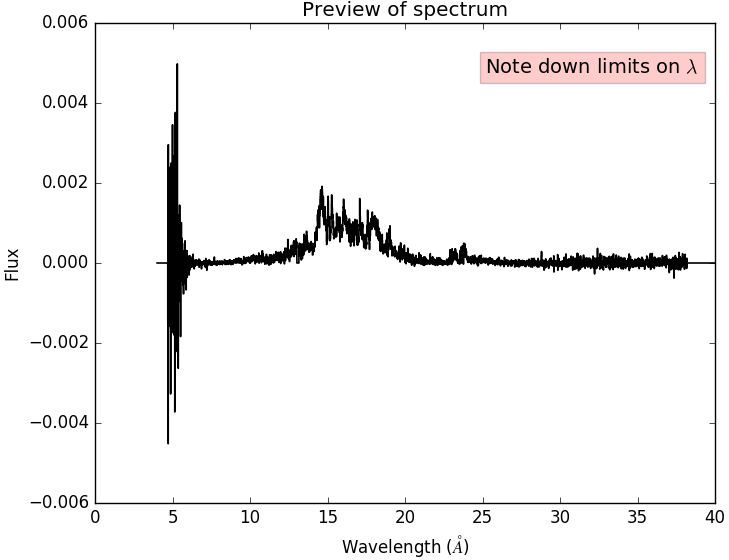
\includegraphics[width=0.9\textwidth]{images/mrvel_preview}
    				\caption{Preview of fluxed spectrum}
    				\label{fig:spec-preview}
			    \end{figure}
			    
			    As it can be seen from the preview in figure \ref{fig:spec-preview}, there seems to be plenty of information in the vicinity of 6 \AA. But this is not usable because it is just noise arising from the low effective area of the RGS instrument in the low wavelength region which severely limits the resolving power of the RGS instrument, as described in the XMM-Newton Users Handbook\footnote{\url{https://xmm-tools.cosmos.esa.int/external/xmm_user_support/documentation/uhb/node1.html}} \cite{xmmUserHandbook}. Also, the region above 26 \AA~has a very low SNR. Looking at the wavelength region between 10 \AA~and 26 \AA~one can clearly visualise a typical spectrum as expected from a luminous X-ray binary source with a good SNR. These wavelength limits are subsequently taken as inputs from the user by the method \texttt{get\_wave\_limits()}.
			 
            \subsubsection{Line list within chosen wavelength range} \label{tool:rgs-files:demonstration:linelist}
                One needs the line list from the NIST database for the given list of ions within a chosen wavelength range. To achieve this, a method called \texttt{get\_lines()} is provided. This takes, as input arguments, the lower and upper wavelength values (in \AA). It uses the list of ions provided in the file \texttt{ion.list}, which is accessed by the script using the \texttt{ASTRODAT} environment variable. Then it queries the NIST database using the \texttt{astroquery.nist.Nist.query()} method.
                
                The \texttt{get\_lines()} method  returns a list of dictionaries, with each dictionary containing four entries: the wavelength (in \AA), the associated ion, a boolean flag which indicates whether that line needs to be included and the colour with which the line is to be plotted. The colour of a line for a specific ion is obtained from another method called \texttt{get\_colour()}. This method uses a pre-defined dictionary of colour maps, from which a colour for a particular ion stage is sampled with the help of a \texttt{NumPy} array. One may add more colour maps corresponding to other ions which may not be included in the code at present.
                
                This method has two more default arguments that allow the user to provide a Doppler shift and to filter out ground level transitions. These arguments are as follows:
                
                \begin{enumerate}[i.]
                    \item An argument \texttt{v\_radial} to provide a radial velocity $v_\text{rad}$ (in km/s), which is then used to compute the Doppler-shifted position $\lambda$ of the line at $\lambda_0$ as
                    \begin{equation}
                        \lambda=\left( 1+\dfrac{v_\text{rad}}{c} \right)\lambda_0 \label{eqn-doppler-shift}
                    \end{equation}
                    The default value of this argument is 0.
                    
                    \item A flag named \texttt{ground\_transitions\_only} which ensures that only those lines are considered which are a consequence of transitions into/from the ground level of the individual ion. The default value of this argument is \texttt{True}, which greatly reduces the density of lines being taken into account.
                \end{enumerate}
            
            \subsubsection{Line-overlaid spectrum} \label{tool:rgs-files:demonstration:lineoverlay}
                Having read the FITS file containing the fluxed spectrum and queried the line list from NIST, one can then proceed to produce a plot of the spectrum, along with the lines overlaid on it. This can be done using the \texttt{plot\_spectrum()} method. This method takes, as input arguments, the lists containing the wavelengths, the fluxes, the errors in the flux, the line list and the lower and upper limits of wavelength.
                
                \begin{figure}[h!]
    				\centering
    				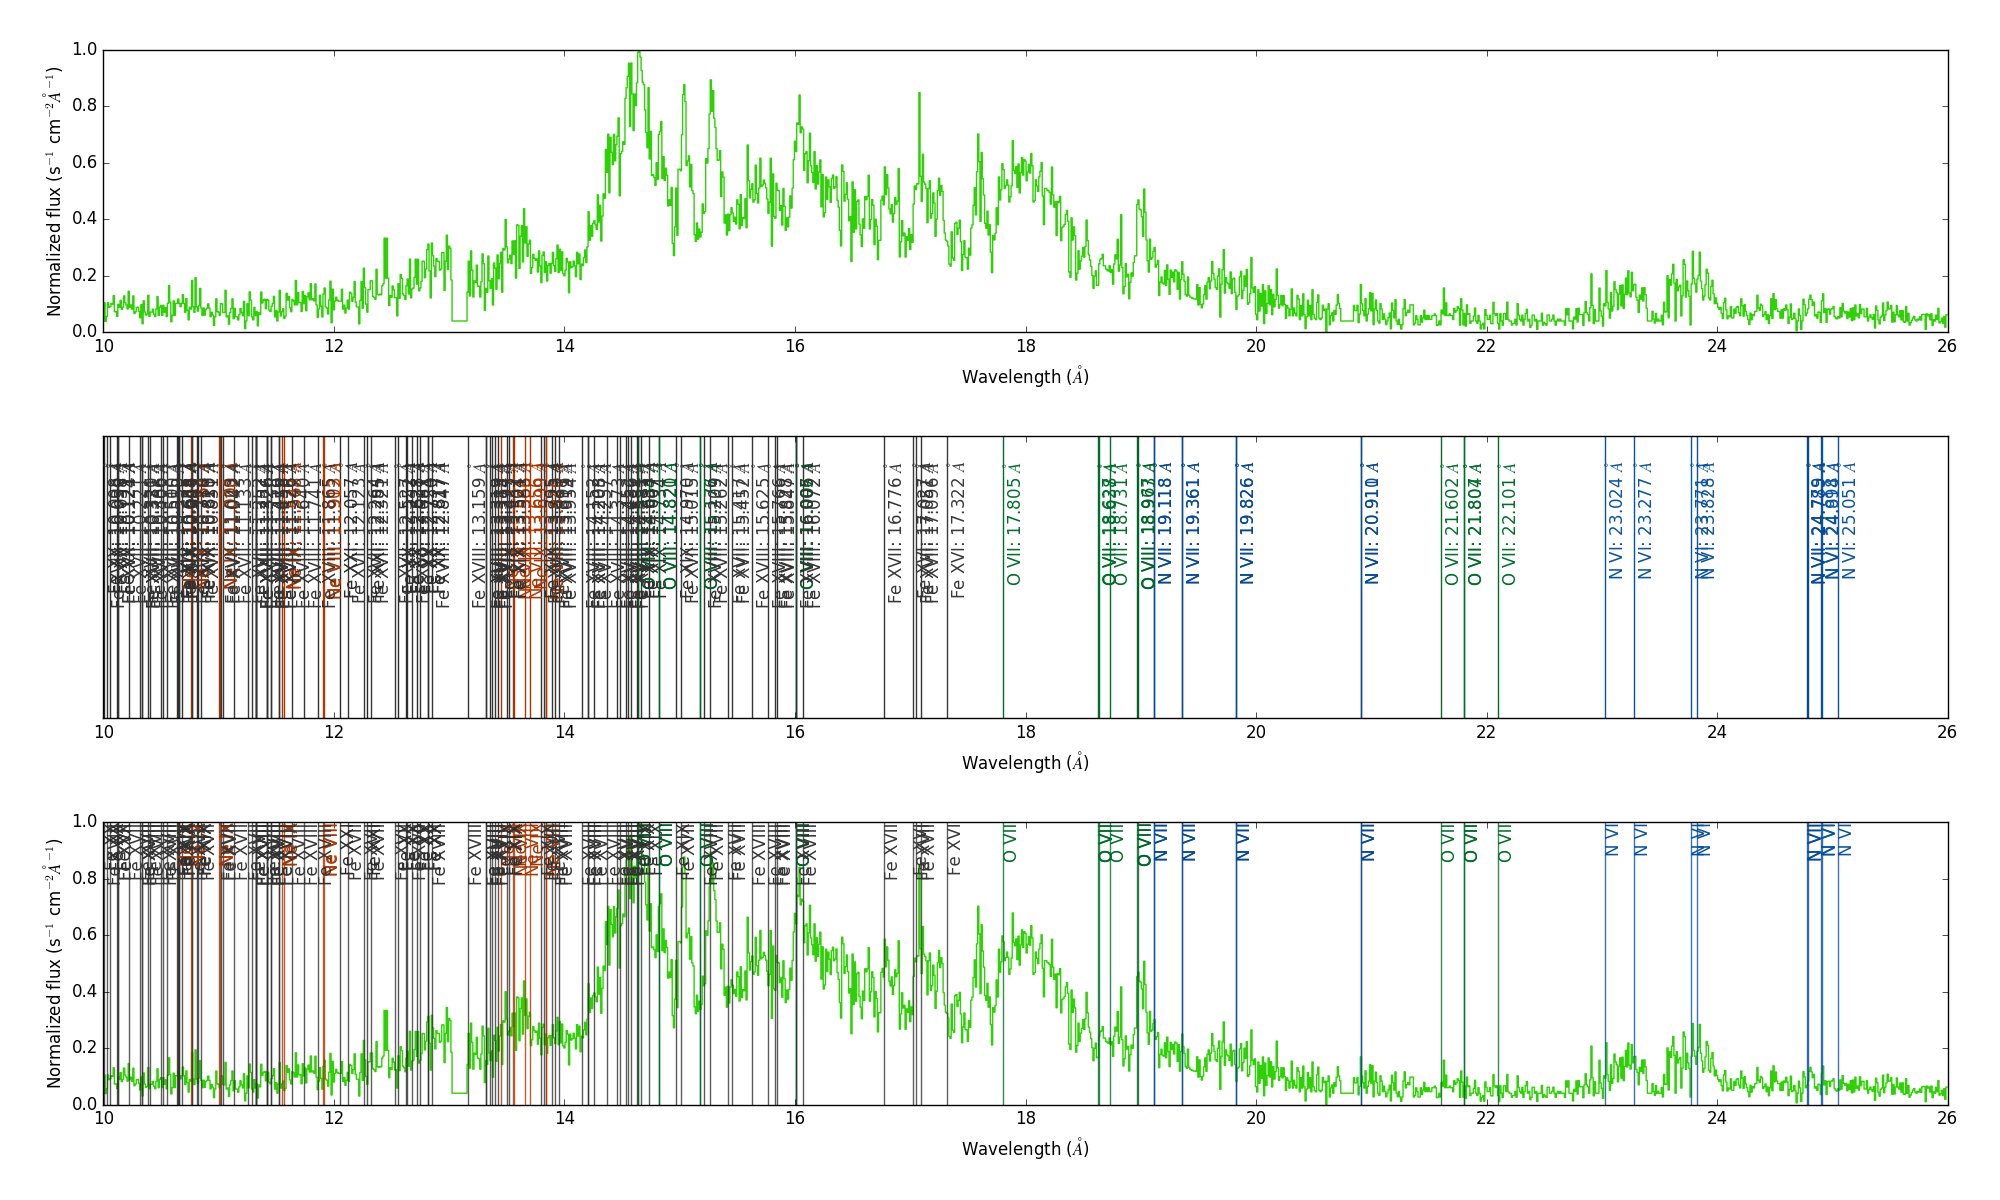
\includegraphics[width=\textwidth]{images/mrvel_line-overlay}
    				\caption{Line-overlaid spectrum using the \texttt{plot\_spectrum()} method}
    				\label{fig:line-overlay}
			    \end{figure}
                
                This method produces a set of three subplots: a plot of the spectrum only, a map of the lines within the wavelength region and a plot of the spectrum with the pertinent lines overlaid. The output of this code for the fluxed spectrum of RX J0925.7-4758 is shown in figure \ref{fig:line-overlay}. As expected, one can observe a profusion of spectral lines due to K-shell transitions of N and O, and due to L-shell transitions of the heavier element Fe. Such an overlay of spectral lines provides a grid of markers of prominent lines. But the actual presence of any line in the spectrum may be latched on to after a closer inspection of sub-regions, as described in \S\ref{tool:rgs-files:demonstration:roi}.
                
                Prior to running the \texttt{plot\_spectrum()} method, one may also choose to display the wavelength values (in \AA) along with the ion label, using the boolean flag \texttt{show\_wavelen- gth} input argument, whose default value is \texttt{False}.
                
                One may also choose to normalize the fluxed spectrum to the range $[0, 1]$ in s$^{-1}$cm$^{-2}$\AA$^{-1}$ using the method \texttt{normalize()}, which takes a list of floats as input and returns another list of floats normalized appropriately. This is helpful in comparing the relative strengths of different lines.
            
            \subsubsection{Inspecting regions of interest} \label{tool:rgs-files:demonstration:roi}
                While the previous method described produces the entire spectrum with overlaid lines, it can be more helpful if one could precisely zoom into any specific region of interest, say between 16.5 \AA~and 18.4 \AA. This can be done with the \texttt{examine\_ROI()} method, which takes the lists of wavelengths, fluxes and errors, the line list, the chosen wavelength range and the lower and upper wavelengths (in \AA) of the region of interest (e.g. 16.5 and 18.4).
                
                \begin{figure}[h!]
    				\centering
    				\includegraphics[width=\textwidth]{images/mrvel_rois}
    				\caption{Partitioning of the fluxed spectrum within specific regions of interest}
    				\label{fig:roi}
			    \end{figure}
                
                Such an inspection of specific regions of interest was carried out for RX J0925.7-4758 and the resulting plots are shown in figure \ref{fig:roi}. One can observe here, for instance, two lines (one due to Fe XVII and the other due to O VIII) nearly overlapping with an emission line in the spectrum around 16.03  \AA. Further analysis of the flux of other lines due to both atomic species would resolve this ambiguity.
                
            \subsubsection{Doppler shifts of lines} \label{tool:rgs-files:demonstration:doppler}
                The emitting matter in stellar sources often have a radial velocity along the line-of-sight because of which their atomic lines often exhibit a Doppler shift, which translates the lines either blue-ward (i.e. towards smaller wavelengths) if the radial velocity is negative (moving towards the observer) or red-ward (i.e. towards larger wavelengths) if the radial velocity is positive (moving away from the observer).
                
                This shift in the wavelength of a line can be obtained as
                
                \begin{equation}
                    \Delta\lambda=\lambda-\lambda_0 \label{eqn-doppler-02}
                \end{equation}
                
                where $\lambda_0$ is the central wavelength of the line and $\lambda$ is the apparent position of the same line. The relation between these two is given by equation \ref{eqn-doppler-shift}. By measuring the $\Delta\lambda$ value from the spectrum for some prominent and well-known atomic lines, one can estimate the radial velocity of the stellar matter which has produced the given spectrum.
                
                One can make an initial estimate of the Doppler shift by plotting the vicinity of a specific line by transforming the horizontal  axis from $\lambda$ (in \AA) to  (in km/s). Then $v_\text{rad}$ is obtained by inverting equation \ref{eqn-doppler-shift} as
                
                \begin{equation}
                    v_\text{rad}=\left( \dfrac{c}{\lambda_0} \right)(\lambda-\lambda_0) \label{eqn-vrad}
                \end{equation}
                
                A method named \texttt{waveshift\_to\_velocity()} is defined which returns $v_\text{rad}$ in km/s, given $\lambda_0$ and $\lambda$ in \AA~as input arguments.
                
                The method named \texttt{plot\_doppler\_lines()} can be used to plot the relative flux of different lines for a specific ion with respect to $v_\text{rad}$. At present, this method can handle the Lyman $\alpha$, $\beta$, and $\gamma$ lines for the H-like and He-like C, N and O ions, as well as some common lines of Fe XVII and Fe XVIII. The list of these lines is given in table \ref{tab:line-list}.
                
                \renewcommand{\arraystretch}{1.2}
                \begin{table}[h!]
                    \centering
                    \caption{List of lines along with transitions, considered for inspection with respect to the radial velocity}
                    \label{tab:line-list}
                    \begin{tabular}{ccc}
                        \hline
                        \textbf{Ion} & \textbf{Transition} & \textbf{Wavelength (in \AA)} \\ \hline
                        \multirow{3}{*}{C V}      & {Ly $\alpha$} & {40.2678} \\ %\cline{2-3} 
                                                  & {Ly $\beta$}  & {34.9728} \\ %\cline{2-3} 
                                                  & {Ly $\gamma$} & {33.4262} \\ \hline
                        \multirow{3}{*}{C VI}     & {Ly $\alpha$} & {33.7396} \\ %\cline{2-3} 
                                                  & {Ly $\beta$}  & {28.4663} \\ %\cline{2-3} 
                                                  & {Ly $\gamma$} & {26.9901} \\ \hline
                        \multirow{3}{*}{N VI}     & {Ly $\alpha$} & {28.7870} \\ %\cline{2-3} 
                                                  & {Ly $\beta$}  & {24.8980} \\ %\cline{2-3} 
                                                  & {Ly $\gamma$} & {23.7710} \\ \hline
                        \multirow{3}{*}{N VII}    & {Ly $\alpha$} & {24.7846} \\ %\cline{2-3} 
                                                  & {Ly $\beta$}  & {20.9106} \\ %\cline{2-3} 
                                                  & {Ly $\gamma$} & {19.8261} \\ \hline
                        \multirow{3}{*}{O VII}    & {Ly $\alpha$} & {21.6020} \\ %\cline{2-3} 
                                                  & {Ly $\beta$}  & {18.6270} \\ %\cline{2-3} 
                                                  & {Ly $\gamma$} & {17.7680*} \\ \hline
                        \multirow{3}{*}{O VIII}   & {Ly $\alpha$} & {18.9725} \\ %\cline{2-3} 
                                                  & {Ly $\beta$}  & {16.0067} \\ %\cline{2-3} 
                                                  & {Ly $\gamma$} & {15.1765} \\ \hline
                        \multirow{3}{*}{Fe XVII}  & {2s$^2$2p$^6$ $\longrightarrow$ 2s$^2$2p$^5$3d} & {15.2620} \\ %\cline{2-3} 
                                                  & {2s$^2$2p$^6$ $\longrightarrow$ 2s$^2$2p$^5$(2P$^o_{3/2}$)3s} & {17.0510} \\ %\cline{2-3} 
                                                  & {2s$^2$2p$^6$ $\longrightarrow$ 2s$^2$2p$^5$(2P$^o_{1/2}$)3s} & {16.7760} \\ \hline
                        \multirow{3}{*}{Fe XVIII} & {2s$^2$2p$^5$ $\longrightarrow$ 2s$^2$2p$^4$(1D)3d} & {14.2080} \\ %\cline{2-3} 
                                                  & {2s$^2$2p$^5$ $\longrightarrow$ 2s$^2$2p$^4$(3P)3d} & {14.3730*} \\ %\cline{2-3} 
                                                  & {2s$^2$2p$^5$ $\longrightarrow$ 2s$^2$2p$^4$(3P)3s} & {16.0050*} \\ \hline
                    \end{tabular}
                    \begin{minipage}{16cm}
						\vspace{0.1cm}
						\small $^*$ Obtained from the Chianti database \cite{dere1997chianti}
					\end{minipage}
                \end{table}
                \renewcommand{\arraystretch}{2.2}
                
                \begin{figure}[!htb]
    				\centering
    				\includegraphics[width=0.8\textwidth]{images/mrvel_N-lines}
    				\caption{Velocity profiles of the Lyman $\alpha$, $\beta$, and $\gamma$ lines for N VI (left) and N VII (right)}
    				\label{fig:vel-prof-N}
			    \end{figure}
			    
			    \begin{figure}[!htb]
    				\centering
    				\includegraphics[width=0.8\textwidth]{images/mrvel_O-lines}
    				\caption{Velocity profiles of the Lyman $\alpha$, $\beta$, and $\gamma$ lines for O VII (left) and O VIII (right)}
    				\label{fig:vel-prof-O}
			    \end{figure}
			    
			    \begin{figure}[!htb]
    				\centering
    				\includegraphics[width=0.8\textwidth]{images/mrvel_Fe-lines}
    				\caption{Velocity profiles of three Fe XVII (left) and Fe XVIII (right) lines}
    				\label{fig:vel-prof-Fe}
			    \end{figure}
                
                Another method named \texttt{map\_spec\_to\_vel()} maps the $\lambda$ values to the  values in the vicinity of a particular line using the previously described methods. It takes as input arguments the central wavelength of the line $\lambda_0$, the lists containing the wavelengths, fluxes and errors, and an argument called \texttt{v\_lim} which defines the bounds of $v_\text{rad}$ values, the default value of which is $\pm$5000 km/s.
                
                Finally, the method named \texttt{plot\_doppler\_lines()} wraps all of these and plots the line profiles for all the lines given in table \ref{tab:line-list}. In case of RX J0925.7-4758, no lines of C V and C VI and also for N VI were detected within the chosen wavelength range. Shown in the figures \ref{fig:vel-prof-N}, \ref{fig:vel-prof-O} and \ref{fig:vel-prof-Fe} are the line profiles obtained for the N VII, O and Fe ions. The \texttt{plot\_doppler\_lines()} method takes, as input arguments, the symbol of the element (`\texttt{C}', `\texttt{N}', `\texttt{O}' or `\texttt{Fe}'), the list of wavelengths, fluxes and errors and the symmetric bound of the radial velocity about 0 (which corresponds to the line centre).
                
                It also takes another argument named mode which serves to draw a dotted vertical line marker either through the lowest flux or the highest flux or both (within the range of radial velocities considered). Either of these options may be chosen by setting \texttt{mode=`abs'} (default value) or \texttt{mode=`ems'} respectively. One can also set \texttt{mode=`Pcyg'} to display both the markers simultaneously. However, one must be cautious while drawing any conclusions about the true position of the line centre from these markers because its position is merely ascertained from the flux values and are meant only to aid the user to get started with an approximate indication about the nature of the shift. For a more accurate evaluation, one needs to rely on a detailed quantitative analysis of the spectrum by using theoretical models.
                
    \subsection{Distribution} \label{tool:rgs-files:distribution}
    	The current version of the entire Python tool is publicly available for download and free use on Github at
    	\begin{center}
    		\url{https://github.com/pararover/xmmrgs_lines}
    	\end{center}
    	By making the code publicly available, critical evaluation and suggestions are desired, which would enable further improvement to the code. Future versions of the code would evolve on the basis of such feedback from an open community.
    	
    \subsection{Future scope} \label{tool:rgs-files:scope}
    	At present, the code is designed to work only with the RGS fluxed spectra from XMM-Newton. While there is no plan to extend its application to binned spectra, it is however planned that future versions of the code would be extended to work on the X-ray spectra from the EPIC MOS and PN instruments of XMM-Newton.
    	
    	Currently, the range of velocity profiles produced by the code is highly restrictive -- it provides the same only for the first three Lyman lines for the H-like and He-like ion stages of C, N, O and Fe only. In future versions, the authors intend to introduce further generalization by allowing the same for any ground transition of any ion, provided any line for the same exists within the chosen wavelength range. The filtering of lines, however, is planned to remain on ground transitions only. The reason for this being that transitions between excited states are much less likely. Also, it is planned that lines could be additionally filtered out on the basis of transition probability -- this would help reduce the cluttering of Fe lines in the lower wavelengths (see the 10 \AA\ -- 16 \AA\ range in figure \ref{fig:line-overlay}).
    
    \section{Stellar Winds from Hot Luminous Massive Stars} \label{tool:stellar-winds}
        Hot luminous massive stars are those with effective temperatures $\sim 10000-50000$ K (i.e. spectral type A0 - O2), luminosities $\sim 10^{37}-10^{39}$ erg/s and masses $\sim 10-50$ M$_\odot$. At the end of their lifetime, such star could collapse as supernovae. If $F$ is the energy flux received at the telescope and $E$ is the energy radiated by the star, knowing the luminosity of such a star one can then use the ratio $\dfrac{F}{E}$ to determine their distances. This enables us to estimate the distances of the galaxies which the stars belong to.
        
        All hot stars with mass $\gtrsim 15$ M$_\odot$ show a high velocity outflow\cite{kudritzki2000winds}. Such an outflow is known as a stellar wind. Consequently, this leads to a mass loss from the star and the winds attaining a terminal velocity owing to Newton's first law of motion. Before proceeding further in the understanding of the driving mechanisms for stellar winds, one needs to be clear of these two important aspects.
        
        \subsection{Mass-Loss Rate} \label{tool:stellar-winds:mass-loss}
        	Due to the outflow of stellar material, the star suffers a mass loss, which is quantified by its \emph{mass-loss rate} $\dot{M}=\dvt{M}{t}$. Typical mass-loss rates of hot stars lie in the range $10^{-7}-10^{-4}$ M$_\odot$/yr, or approximately $\dfrac{1}{30}-30$ M$_\text{earth}$/yr. In comparison, the sun also has a mass outflow, called \emph{solar wind}, with $\dot{M}\approx 10^{-14}$ M$_\odot$/yr.
        
        \subsection{Terminal Velocity} \label{tool:stellar-winds:term-vel}
        	When stellar material is far from the surface of the star, it reaches its maximum velocity owing to the acceleration from the radiation pressure. At such large distances, due to the absence of any other external forces, the stellar velocity remains constant as per Newton's first law of motion. Therefore, this constant maximum velocity is known as the terminal velocity $v_\infty$.
        	
        	Typical values for $v_\infty$ lie between $\sim 200$ km/s (for A-type supergiants) and $\sim 3000$ km/s (for early O-type stars). Consequently, the speed of sounds in such atmospheres varies between 10 km/s to 30 km/s as per the relation:
        	\begin{align*}
        		V(R)=v_\infty\left(1-b\dfrac{R_*}{R}\right)^\beta
        	\end{align*}
	
	\section{Relevance of Stellar Winds} \label{tool:relevance}
		The analysis of stellar winds gains importance due to the reasons outlined below:
		\begin{itemize}
			\item The lifetime of hot stars is approximately $10^{-3}$ that of the sun, i.e. $\sim 10^7$ yr. Assuming $\dot{M}\sim 10^{-6}$ M$_\odot$/yr, the mass loss due to stellar winds is $\sim 10^7$ yr $\times 10^{-6}$ M$_\odot$/yr $\approx 10$ M$_\odot$ during its entire lifetime. This is a significant mass loss, e.g. for a star with an initial mass of $20$ M$_\odot$, half of its mass is lost due to stellar winds. Therefore, in order to have an accurate picture of the \emph{evolution of hot stars}, it is essential to know its mass loss rate, and hence the stellar wind.
			\item In the interior of stellar cores, for most part of the star's lifetime energy is generated by the CNO bi-cycle. Therefore, the abundance ratio of the elements $\text{H}:\text{He}:\text{C}:\text{N}:\text{O}$ is altered during the stellar lifetime, as compared to that during its birth. Furthermore, the nuclear processed matter is transported to the outer regions of the star by diffusion and convection, to be eventually carried to the surrounding space by the stellar wind. Because the hot stars are almost always clumped together in groups, these processes may significantly impact the chemical composition of the ISM, thereby affecting the \emph{galactic evolution}.
			\item Far away from hot stars, where the stellar wind attains supersonic terminal velocities, it may collide with the surrounding material, leading to the development of shocks, which may lead to local compressions in the surrounding material. This may trigger the formation of proto-stars, leading to the birth of new stars. Therefore, the \emph{formation of new stars} could be affected by the presence of stellar winds due to hot stars.
		\end{itemize}
	
	\section{Radiative Line-Driving: Mechanism of Stellar Winds} \label{tool:radiative-line-driving}
		The physical mechanism which initiates and drives the outflow of matter from hot stars is known as radiative line driving. Given below is a qualitative description of the physical mechanism behind this process.
		\begin{figure}[h!]
			\centering
			\subfloat[Absorption of photon \label{rad-line-drive:absorption}]{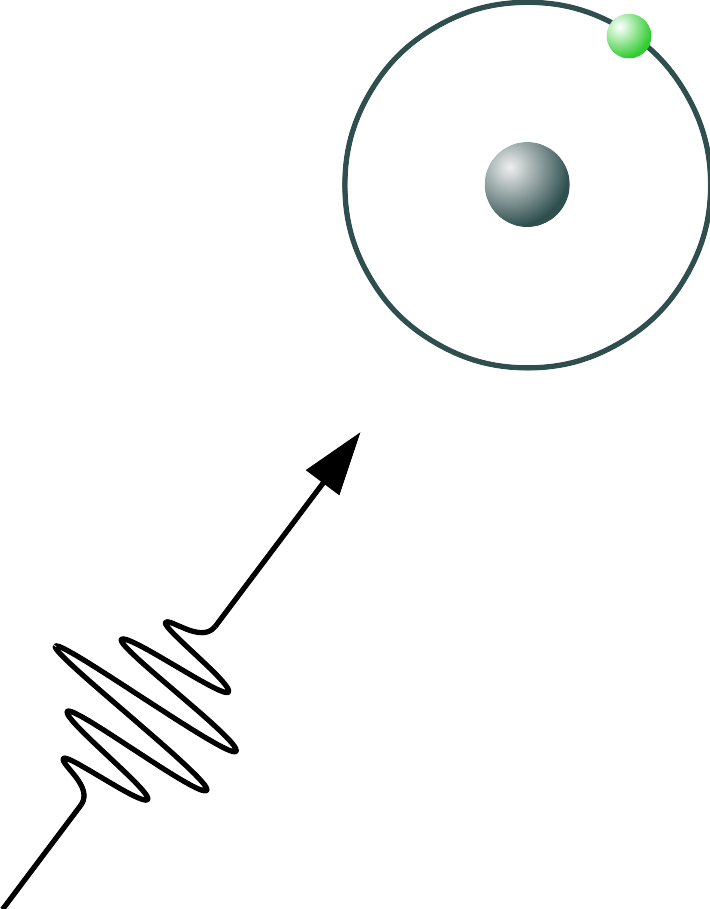
\includegraphics[scale=0.7]{rad-line-drive-01}} \hfill
			\subfloat[Excitation of atom \label{rad-line-drive:excitation}] {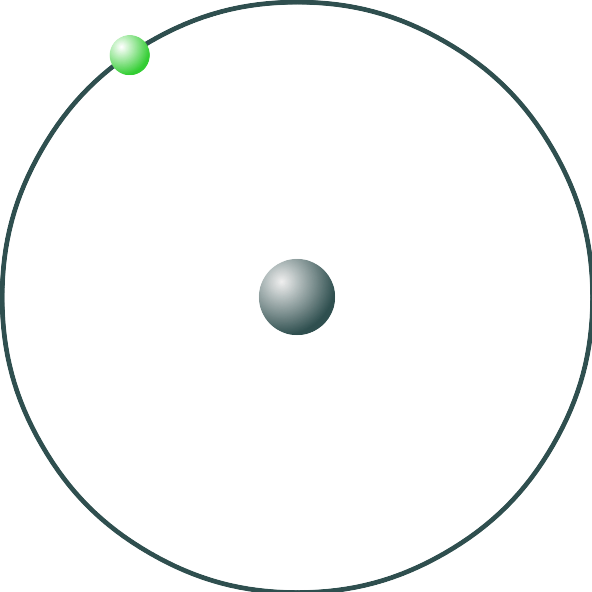
\includegraphics[scale=0.7]{rad-line-drive-02}} \hfill
			\subfloat[Re-emission of photon \label{rad-line-drive:reemission}] {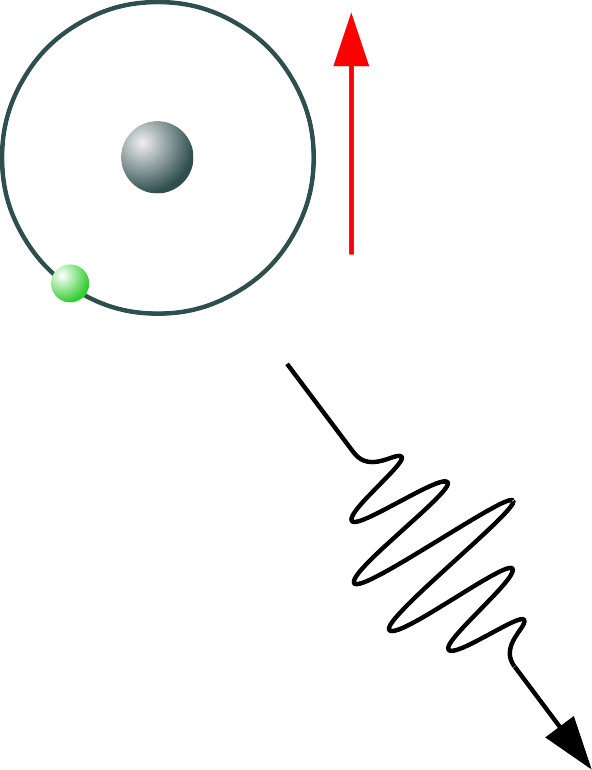
\includegraphics[scale=0.8]{rad-line-drive-03}}\\ %\hfill
			\caption{Principle of radiative line driving}
			\label{rad-line-drive-principle}
		\end{figure}
		
		\begin{figure}[h!]
			\centering
			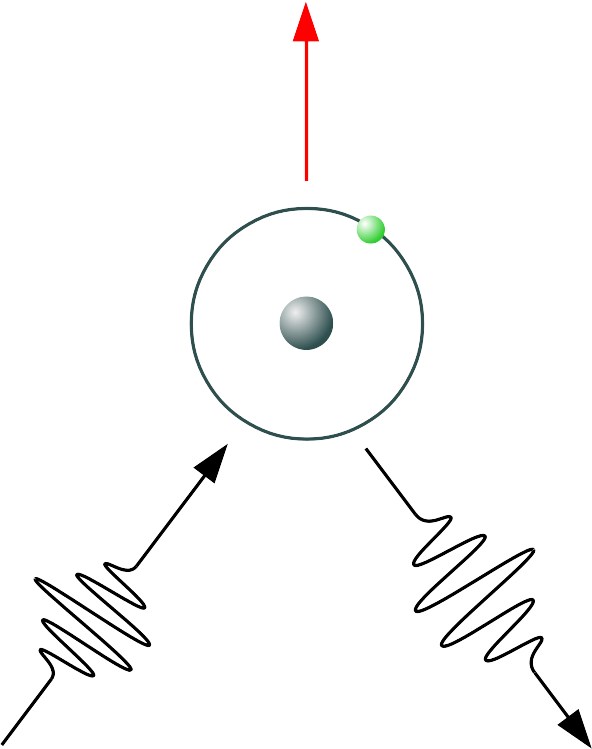
\includegraphics[scale=1.0]{rad-line-drive-04}
			\caption{Momentum transfer during radiative line driving}
			\label{rad-line-drive-momentum}
		\end{figure}
		Figure \ref{rad-line-drive-principle} depicts the interaction between the wind material (comprising of ions) and the photons emitted from the deeper layers of the stellar atmosphere, known as the photosphere. The transfer of momentum from the photons to the ions takes place in three steps:
		\begin{enumerate}[i.]
			\item The absorption of a photon by an ion
			\item The excitation of the ion
			\item The re-emission of a photon by the ion
		\end{enumerate}
